\documentclass[12pt,a4paper]{article}
\usepackage[utf8]{inputenc}
\usepackage[T1]{fontenc}
\usepackage[polish]{babel}
\usepackage{amsmath, amsfonts, geometry, fancyhdr, graphicx, float, booktabs, caption, subcaption}

\geometry{margin=2.5cm}
\graphicspath{{./}}

\pagestyle{fancy}
\fancyhf{}
\lhead{Piotr Sączawa}
\rhead{Data: \today}
\chead{MOwNiT - Laboratorium 8}
\cfoot{\thepage}

\begin{document}

\begin{center}
    \section*{Rozwiązywanie równań różniczkowych zwyczajnych}
\end{center}

\subsection*{1. Wstęp i opis problemu}

Celem ćwiczenia jest numeryczne rozwiązanie równania różniczkowego zwyczajnego pierwszego rzędu oraz porównanie jakości aproksymacji otrzymanej dwiema metodami:
\begin{itemize}
    \item jawną metodą Eulera,
    \item klasyczną metodą Rungego-Kutty czwartego rzędu.
\end{itemize}

Badane równanie ma postać
\begin{equation}
    y' - k m y \sin(mx) = k^2 m \sin(mx)\cos(mx), \qquad y(x_0)=a.
    \label{eq:ode}
\end{equation}

Dla tego równania znane jest rozwiązanie analityczne
\begin{equation}
    y(x) = e^{-k\cos(mx)} - k\cos(mx) + 1.
    \label{eq:exact}
\end{equation}

W eksperymencie wykorzystano indywidualne parametry
\begin{equation}
    k=8, \qquad m=1, \qquad x \in \left[\frac{3}{2}\pi, 3\pi\right].
\end{equation}

Warunek początkowy dobrano z rozwiązania dokładnego. Ponieważ
\begin{equation}
    y\left(\frac{3}{2}\pi\right)
    = e^{-8\cos(\frac{3}{2}\pi)} - 8\cos\left(\frac{3}{2}\pi\right) + 1
    = 2,
\end{equation}
przyjęto $x_0=\frac{3}{2}\pi$ oraz $a=2$.

Obliczenia wykonano dla kroków
\begin{equation}
    h \in \{10^{-1}, 10^{-2}, 10^{-3}, 10^{-4}, 10^{-5}\}.
\end{equation}

\subsection*{2. Dane techniczne i metodyka badawcza}

\begin{table}[H]
\centering
\begin{tabular}{|l|l|}
\hline
\textbf{Parametr} & \textbf{Specyfikacja} \\ \hline
Język programowania & Python 3.12 \\ \hline
Biblioteki & NumPy, Matplotlib \\ \hline
System operacyjny & Windows 11 / Linux x86\_64 \\ \hline
Procesor & AMD Ryzen 5 5600H \\ \hline
Precyzja obliczeń & Zmiennoprzecinkowa podwójna, 64-bitowa \\ \hline
\end{tabular}
\caption{Specyfikacja środowiska obliczeniowego.}
\label{tab:dane_techniczne}
\end{table}

Metoda Eulera została zaimplementowana według wzoru
\begin{equation}
    y_{i+1} = y_i + h f(x_i, y_i),
\end{equation}
gdzie po przekształceniu równania \eqref{eq:ode}
\begin{equation}
    f(x,y) = k m \sin(mx)\left(y + k\cos(mx)\right).
\end{equation}

W metodzie Rungego-Kutty czwartego rzędu użyto klasycznego schematu
\begin{align}
    K_1 &= f(x_i, y_i), \\
    K_2 &= f\left(x_i+\frac{h}{2}, y_i+\frac{hK_1}{2}\right), \\
    K_3 &= f\left(x_i+\frac{h}{2}, y_i+\frac{hK_2}{2}\right), \\
    K_4 &= f(x_i+h, y_i+hK_3), \\
    y_{i+1} &= y_i + \frac{h}{6}(K_1 + 2K_2 + 2K_3 + K_4).
\end{align}

Dla każdego kroku $h$ porównano wartości numeryczne z rozwiązaniem dokładnym \eqref{eq:exact}. Wykresy oraz tabela błędów zostały wygenerowane skryptem \texttt{generate\_results.py}.

\newpage

\subsection*{3. Analiza wyników numerycznych}

\begin{figure}[H]
    \centering
    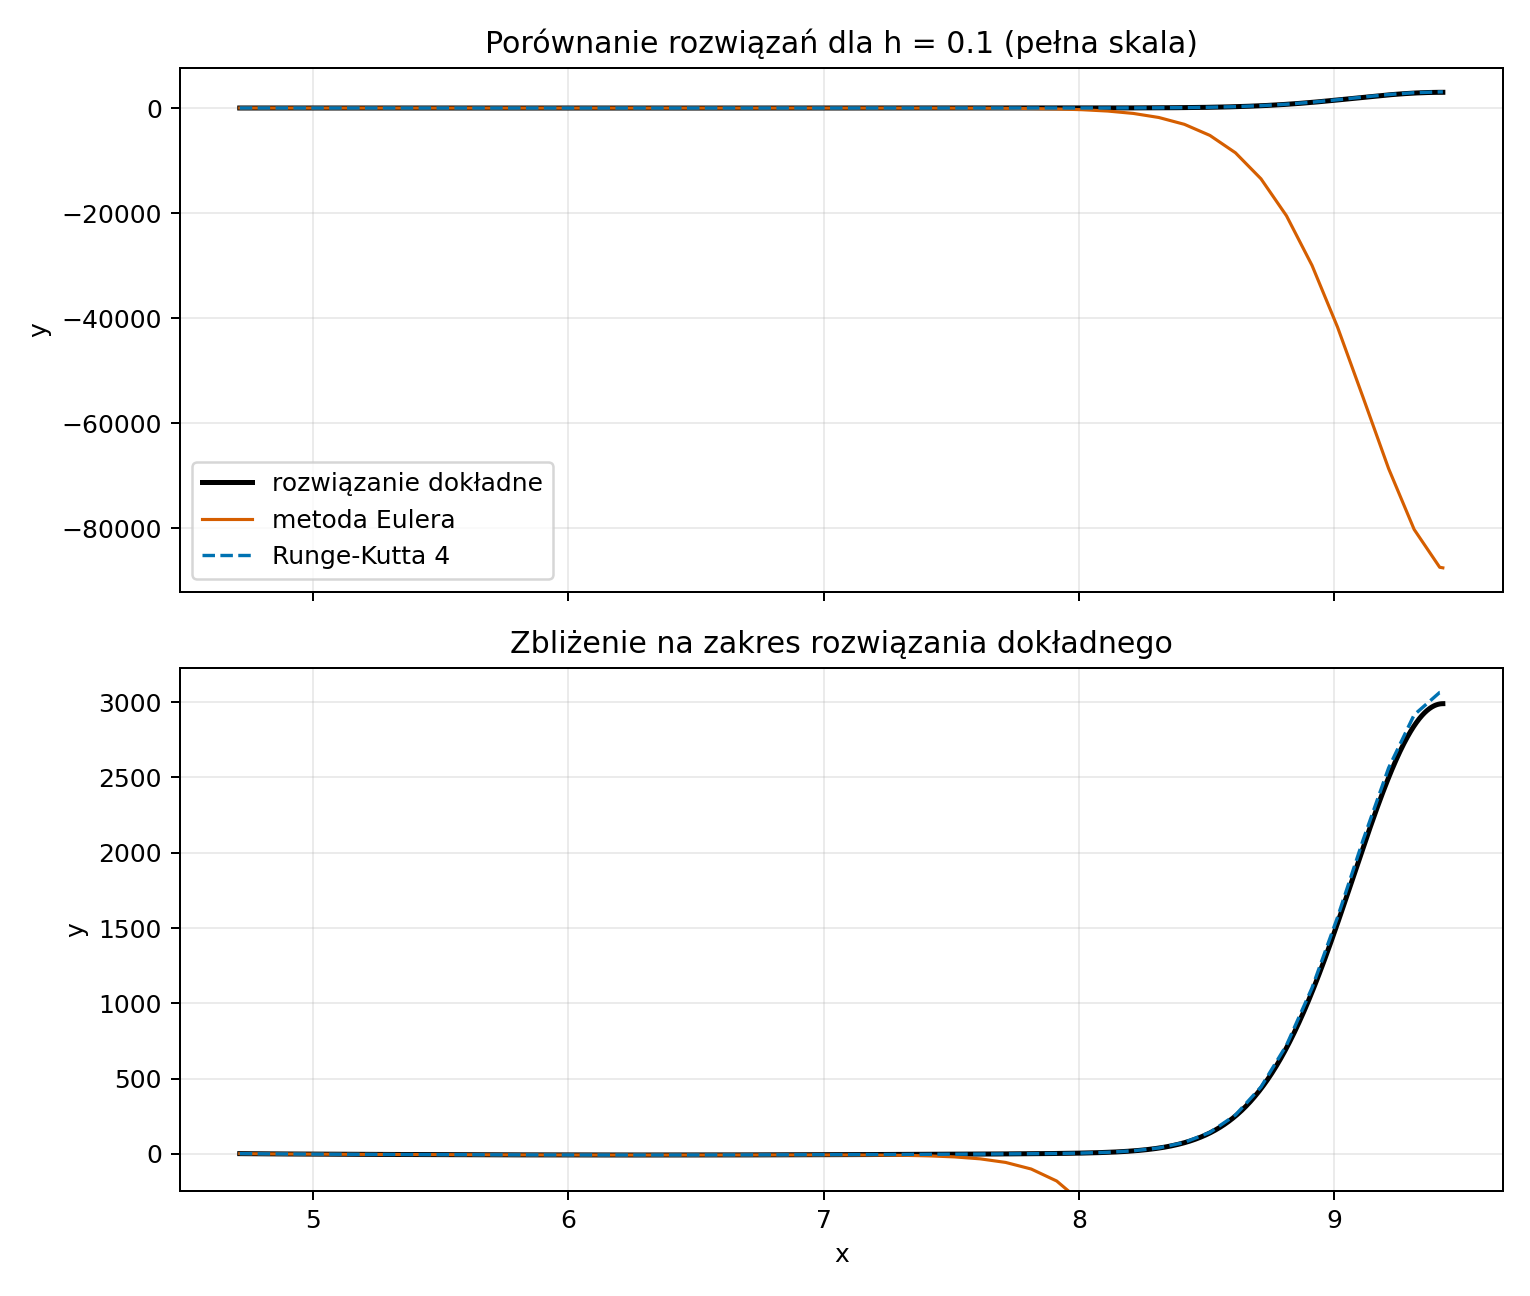
\includegraphics[width=0.82\textwidth]{rozwiazania_h_1e-01.png}
    \caption{Rozwiązanie dokładne oraz aproksymacje dla kroku $h=0.1$.}
    \label{fig:h1}
\end{figure}

Dla największego kroku $h=0.1$ metoda Eulera nie odwzorowuje poprawnie końcowego fragmentu rozwiązania. Górny panel pokazuje pełną skalę błędu tej metody, natomiast dolny panel ułatwia ocenę dopasowania w zakresie rozwiązania dokładnego. Metoda Rungego-Kutty czwartego rzędu zachowuje znacznie lepszą zgodność, lecz także wykazuje zauważalny błąd, ponieważ krok jest nadal duży względem szybkości zmian funkcji.

\begin{figure}[H]
    \centering
    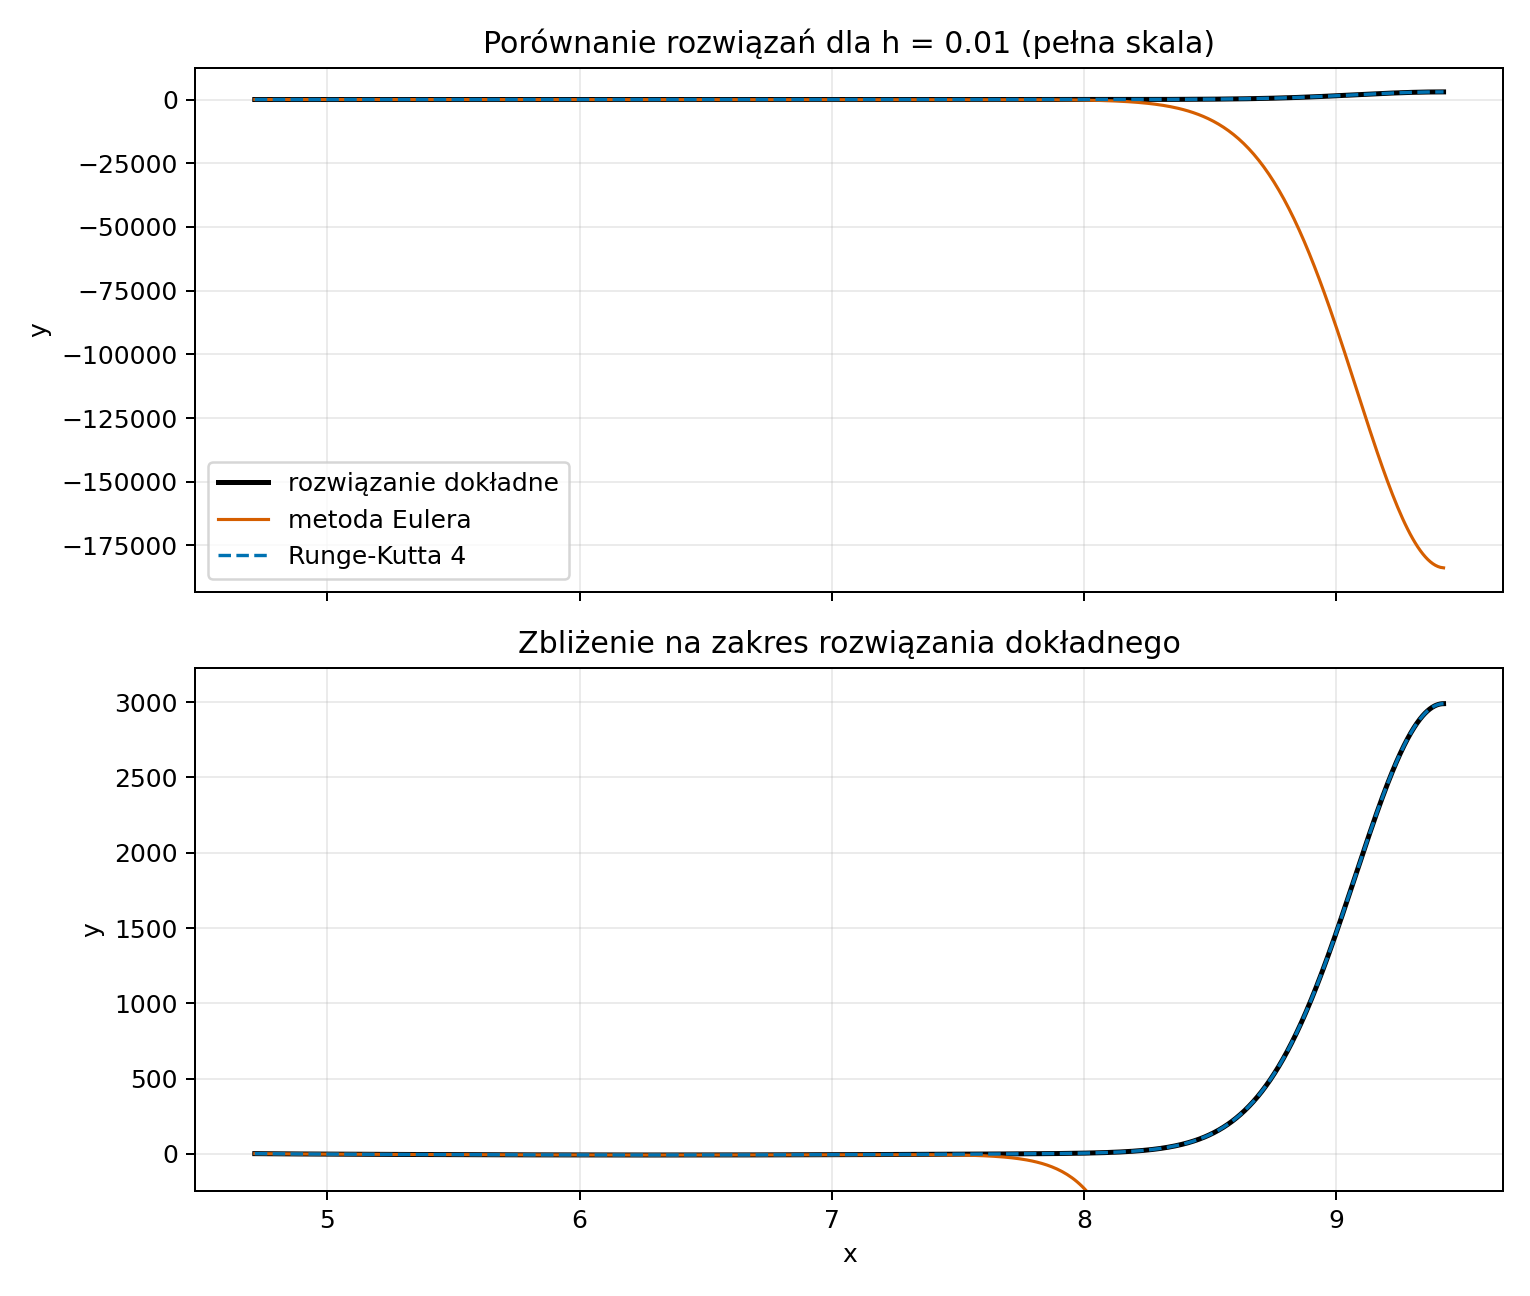
\includegraphics[width=0.82\textwidth]{rozwiazania_h_1e-02.png}
    \caption{Rozwiązanie dokładne oraz aproksymacje dla kroku $h=0.01$.}
    \label{fig:h2}
\end{figure}

Po zmniejszeniu kroku do $h=0.01$ metoda Rungego-Kutty praktycznie pokrywa się z rozwiązaniem analitycznym w zbliżeniu dolnego panelu. W przypadku metody Eulera nadal widoczna jest duża kumulacja błędu globalnego. Jest to przykład sytuacji, w której samo dziesięciokrotne zmniejszenie kroku nie gwarantuje jeszcze proporcjonalnego spadku błędu w całym przedziale, ponieważ błąd z wcześniejszych punktów zostaje wzmocniony przez dynamiczny wzrost rozwiązania.

\begin{figure}[H]
    \centering
    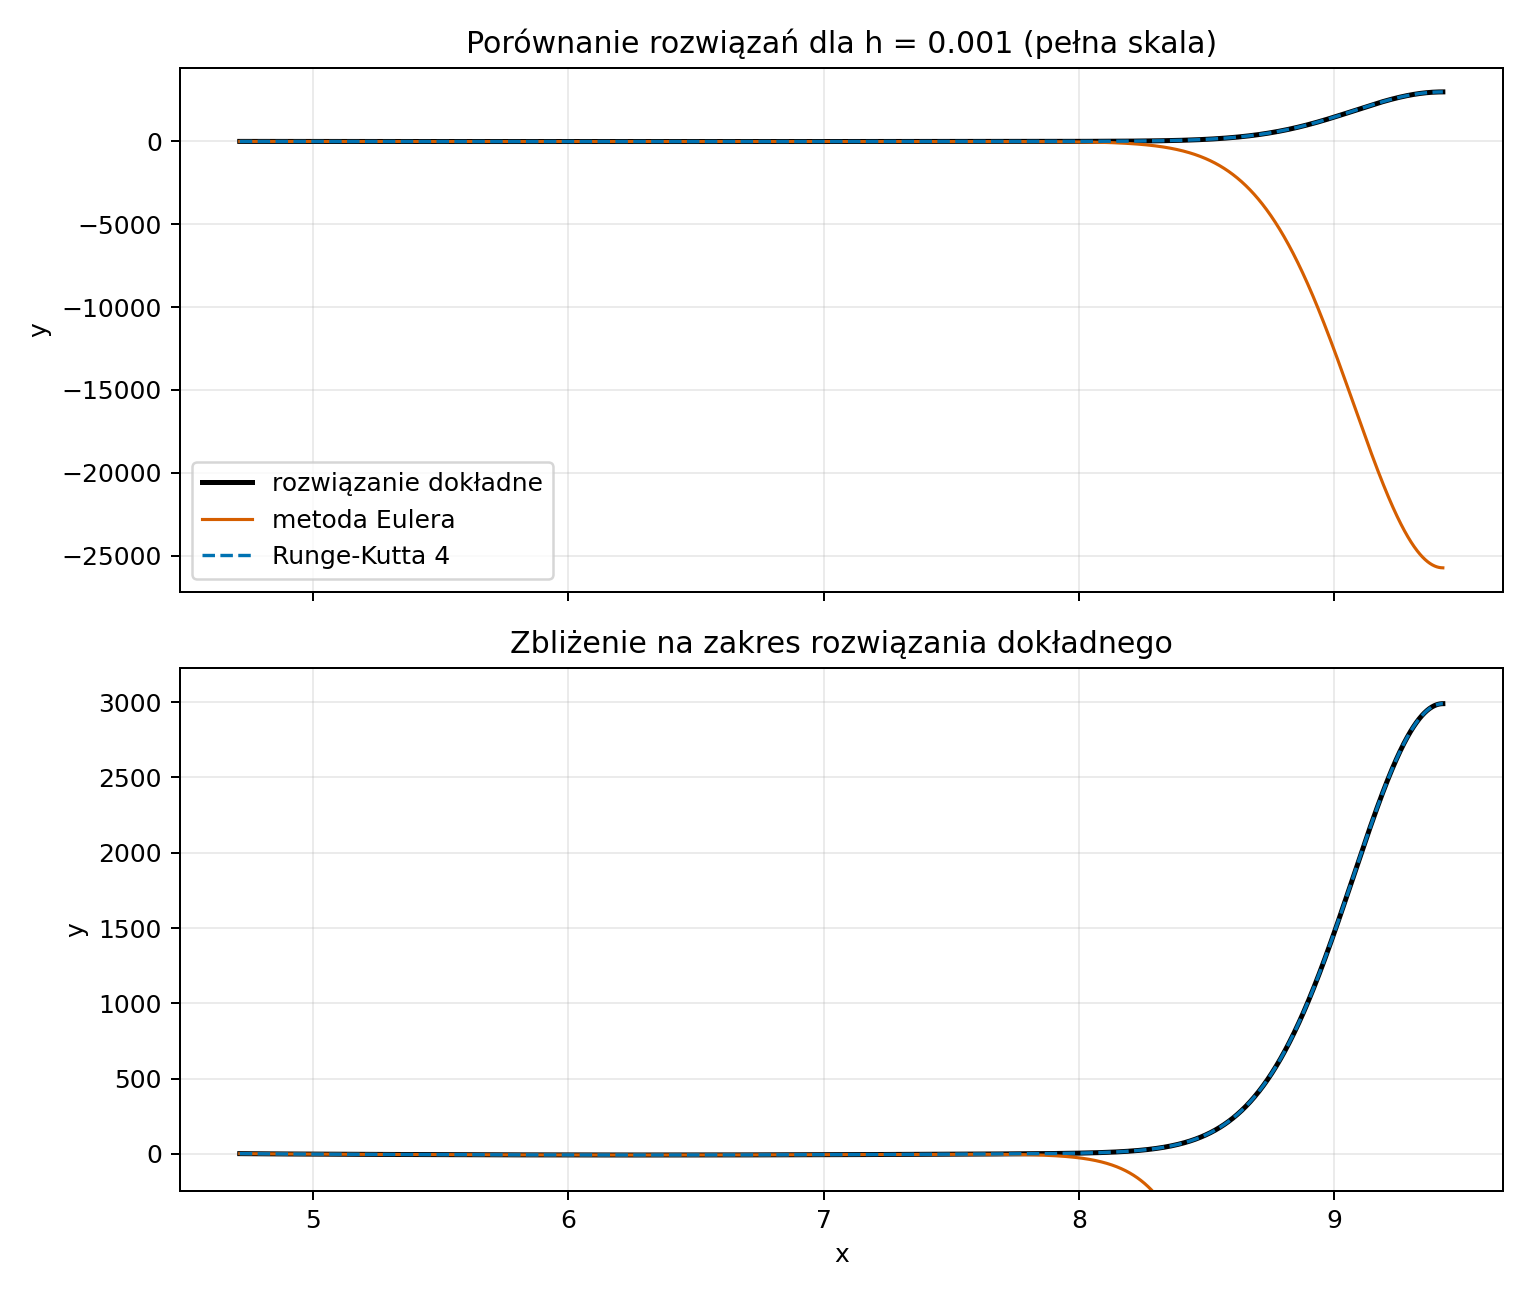
\includegraphics[width=0.82\textwidth]{rozwiazania_h_1e-03.png}
    \caption{Rozwiązanie dokładne oraz aproksymacje dla kroku $h=0.001$.}
    \label{fig:h3}
\end{figure}

Dla $h=0.001$ jakość metody Eulera wyraźnie się poprawia, choć w pobliżu końca przedziału nadal można zauważyć różnicę względem krzywej dokładnej. Metoda Rungego-Kutty pozostaje wizualnie nierozróżnialna od rozwiązania analitycznego.

\begin{figure}[H]
    \centering
    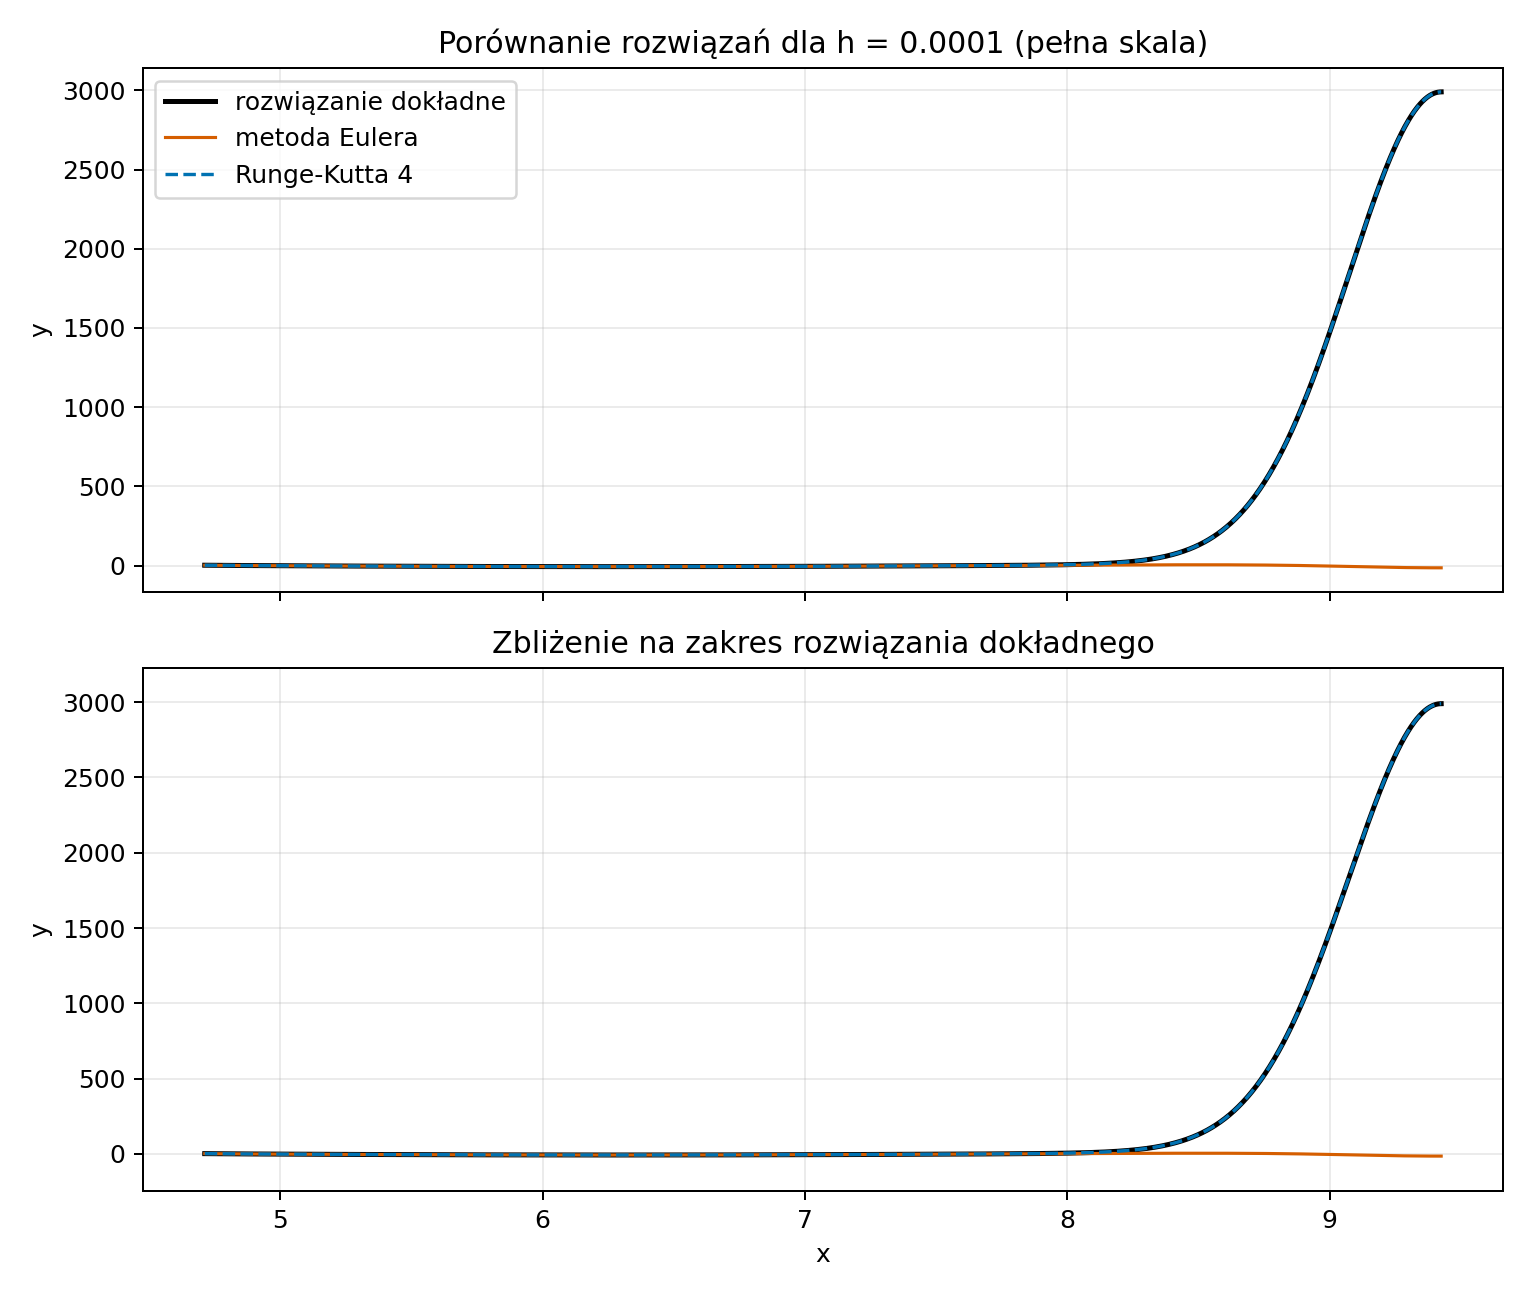
\includegraphics[width=0.82\textwidth]{rozwiazania_h_1e-04.png}
    \caption{Rozwiązanie dokładne oraz aproksymacje dla kroku $h=0.0001$.}
    \label{fig:h4}
\end{figure}

Dla kroku $h=0.0001$ rozwiązanie uzyskane metodą Eulera jest już znacznie bliższe rozwiązaniu dokładnemu, ale nadal obserwowany jest błąd rzędu tysięcy jednostek w skali maksymalnej. Wynika to z faktu, że wartości funkcji na końcu przedziału osiągają poziom około $3\cdot 10^3$, a współczynnik przy $y$ w równaniu powoduje wzmacnianie błędu propagowanego z poprzednich iteracji.

\begin{figure}[H]
    \centering
    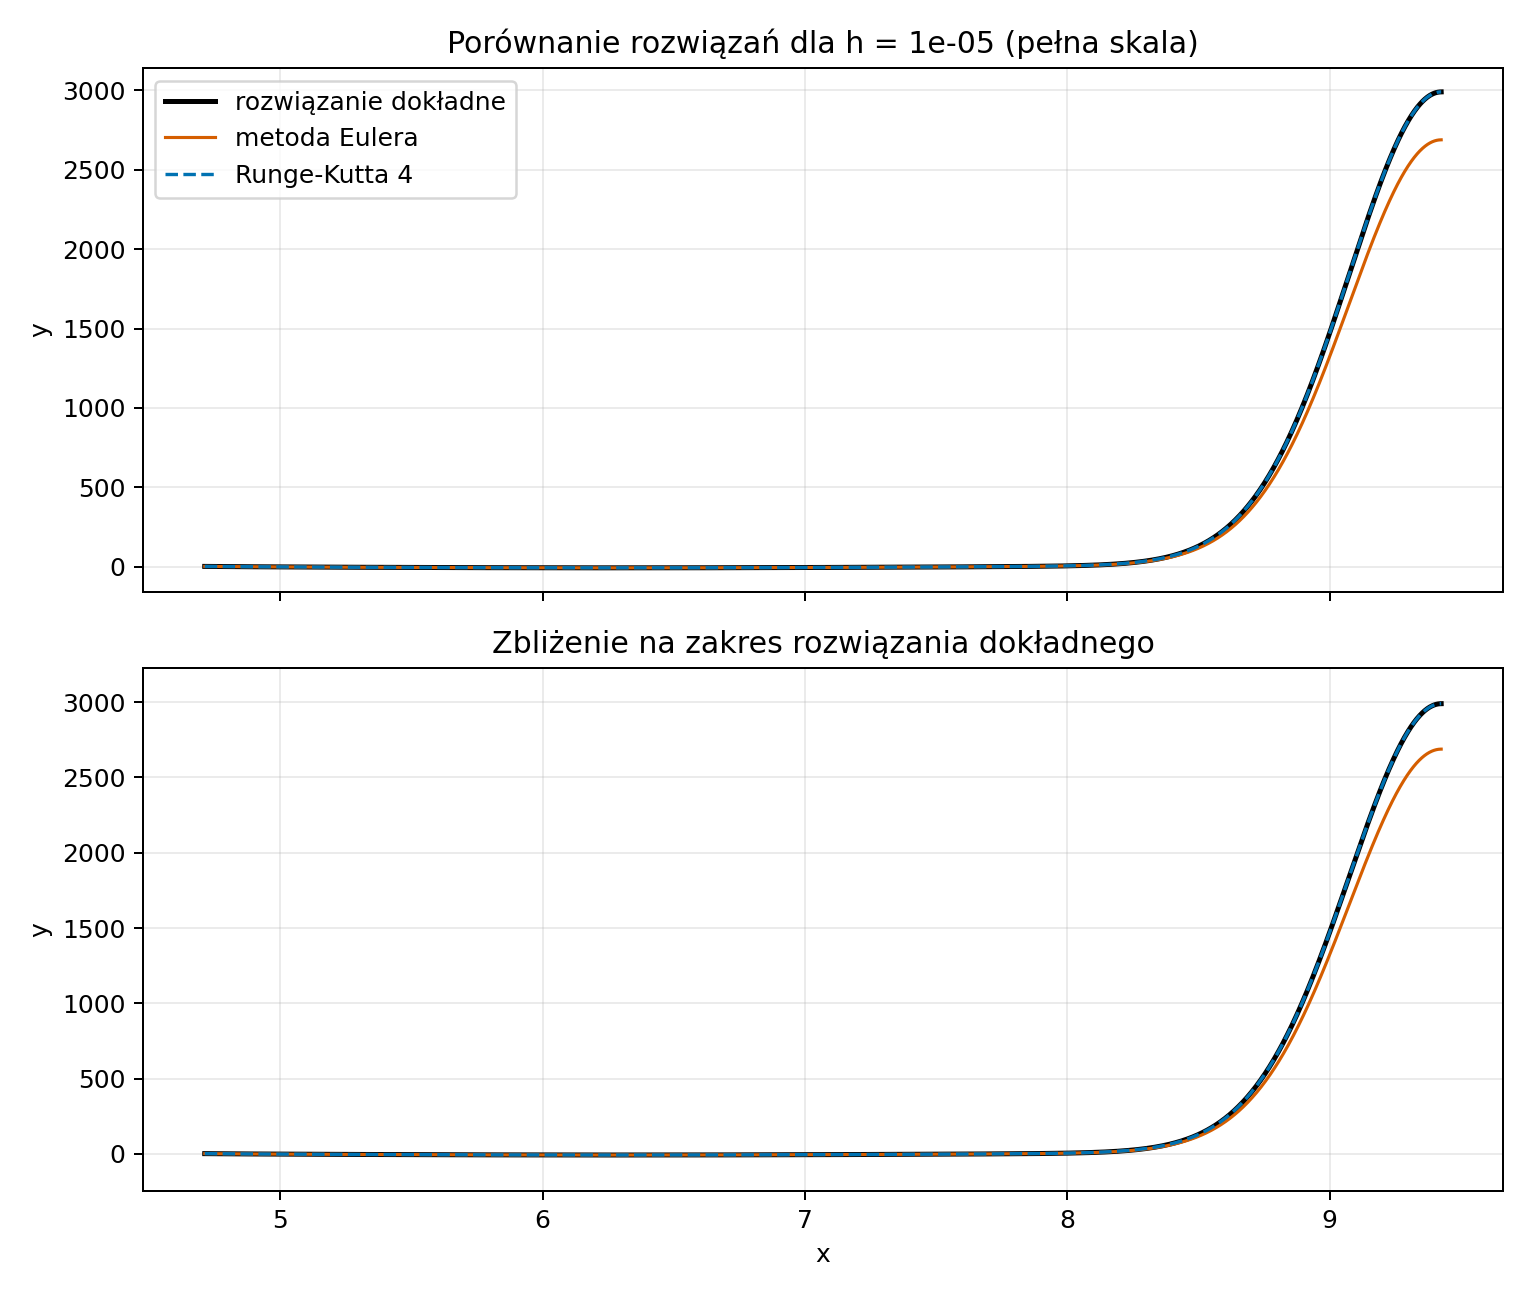
\includegraphics[width=0.82\textwidth]{rozwiazania_h_1e-05.png}
    \caption{Rozwiązanie dokładne oraz aproksymacje dla kroku $h=0.00001$.}
    \label{fig:h5}
\end{figure}

Najmniejszy badany krok $h=0.00001$ daje najlepsze dopasowanie metody Eulera spośród wszystkich przeprowadzonych eksperymentów. Różnica między rozwiązaniem dokładnym a przybliżeniem jest już mała w skali wykresu, natomiast metoda Rungego-Kutty nadal utrzymuje bardzo wysoką dokładność.

\newpage

\subsection*{4. Analiza błędów przybliżenia}

Do oceny jakości wyników zastosowano błąd maksymalny:
\begin{equation}
    E_{\max} = \max_{i \in \{1,2,\dots,l\}} |y_i - \widetilde{y}_i|,
    \label{eq:error}
\end{equation}
gdzie:
\begin{itemize}
    \item $l$ oznacza liczbę punktów siatki,
    \item $y_i$ jest wartością rozwiązania dokładnego w punkcie $x_i$,
    \item $\widetilde{y}_i$ jest wartością otrzymaną badaną metodą numeryczną.
\end{itemize}

\begin{table}[H]
\centering
\begin{tabular}{rcc}
\toprule
$h$ & Metoda Eulera & Metoda Rungego-Kutty \\
\midrule
$10^{-1}$ & $9.04952\cdot 10^{4}$ & $7.63712\cdot 10^{1}$ \\
$10^{-2}$ & $1.86781\cdot 10^{5}$ & $3.09363\cdot 10^{-3}$ \\
$10^{-3}$ & $2.87236\cdot 10^{4}$ & $5.16319\cdot 10^{-7}$ \\
$10^{-4}$ & $3.00441\cdot 10^{3}$ & $1.41816\cdot 10^{-7}$ \\
$10^{-5}$ & $3.01801\cdot 10^{2}$ & $1.06443\cdot 10^{-6}$ \\
\bottomrule
\end{tabular}

\caption{Porównanie błędów maksymalnych $E_{\max}$ dla obu metod.}
\label{tab:bledy}
\end{table}

\begin{figure}[H]
    \centering
    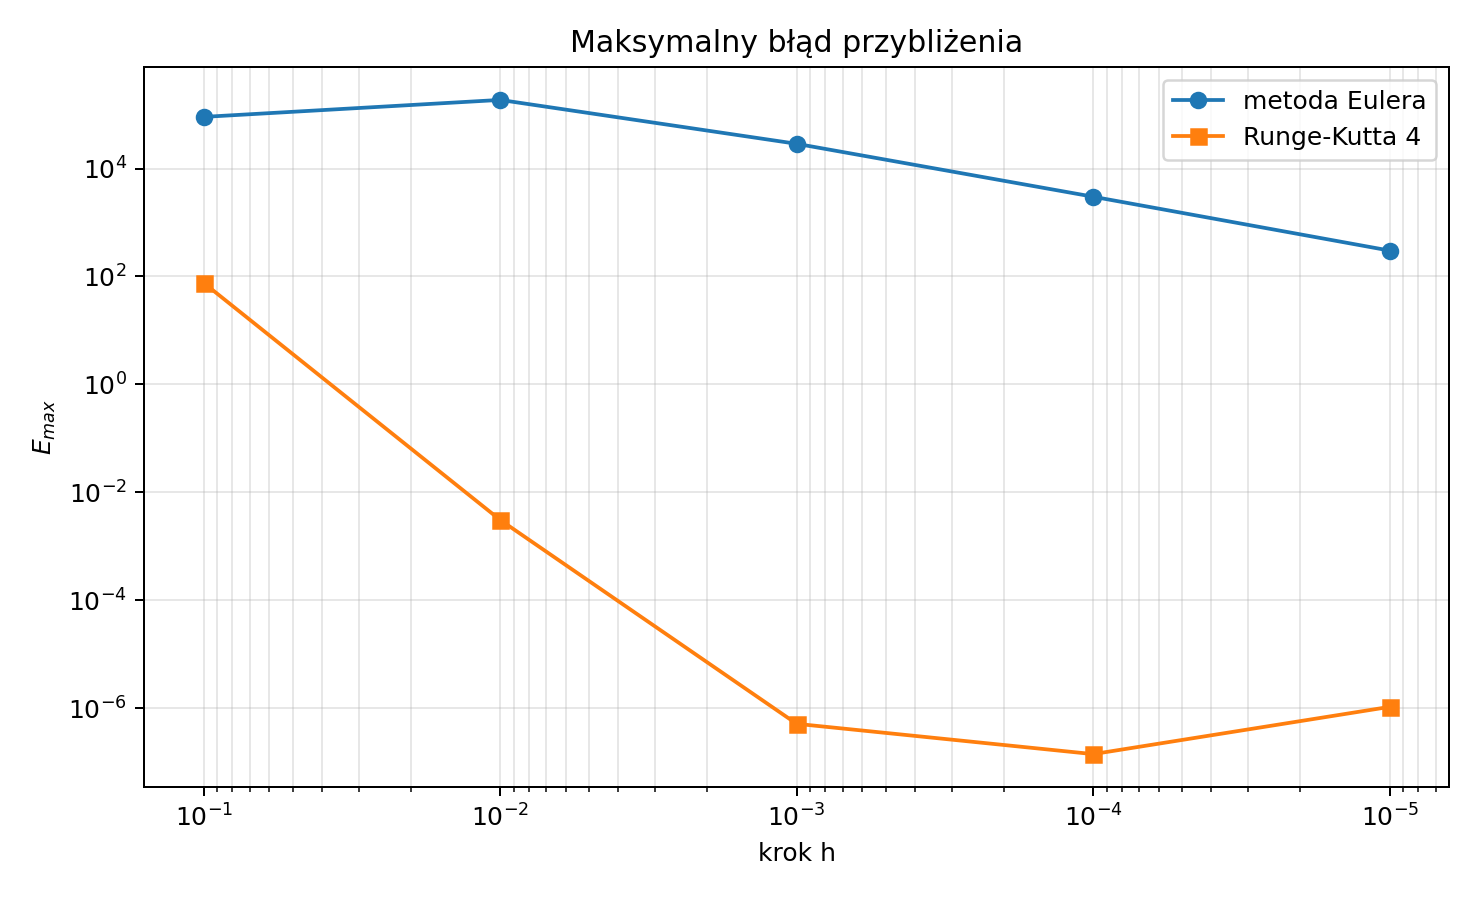
\includegraphics[width=0.86\textwidth]{bledy_maksymalne.png}
    \caption{Zależność błędu maksymalnego od kroku całkowania.}
    \label{fig:bledy}
\end{figure}

Wyniki z Tabeli \ref{tab:bledy} potwierdzają zasadniczą przewagę metody Rungego-Kutty czwartego rzędu nad metodą Eulera. Dla kroku $h=10^{-2}$ błąd RK4 wynosi około $3.09\cdot 10^{-3}$, podczas gdy błąd metody Eulera pozostaje na poziomie $1.87\cdot 10^5$. Oznacza to różnicę wielu rzędów wielkości.

Warto zauważyć, że dla metody Eulera błąd przy $h=10^{-2}$ jest większy niż dla $h=10^{-1}$. Nie jest to sprzeczne z teorią zbieżności, ponieważ teoria opisuje zachowanie asymptotyczne dla dostatecznie małych kroków. W badanym równaniu rozwiązanie silnie rośnie pod koniec przedziału, a jawny schemat Eulera przenosi i wzmacnia wcześniejsze odchylenia. Dopiero dla kroków od $10^{-3}$ w dół widoczny jest systematyczny spadek błędu.

Dla metody Rungego-Kutty oczekiwany spadek błędu jest bardzo szybki. Przy najmniejszych krokach różnice między kolejnymi wynikami są już bliskie ograniczeniom arytmetyki zmiennoprzecinkowej i kumulacji błędów zaokrągleń, dlatego błąd nie maleje idealnie monotonicznie.

\subsection*{5. Wnioski}

\begin{enumerate}
    \item \textbf{Rząd metody ma kluczowe znaczenie.} Metoda Rungego-Kutty czwartego rzędu osiągnęła bardzo wysoką dokładność już dla $h=10^{-2}$, podczas gdy metoda Eulera wymagała znacznie mniejszych kroków, aby wizualnie zbliżyć się do rozwiązania dokładnego.
    \item \textbf{Metoda Eulera jest wrażliwa na propagację błędu.} W badanym przedziale rozwiązanie gwałtownie rośnie przy $x \rightarrow 3\pi$, przez co błędy lokalne z wcześniejszych kroków są mocno wzmacniane w końcowej części obliczeń.
    \item \textbf{Zmniejszanie kroku poprawia dokładność, ale zwiększa koszt obliczeń.} Dla $h=10^{-5}$ liczba kroków jest bardzo duża, a mimo to metoda Eulera pozostaje mniej dokładna niż RK4 dla znacznie większych kroków.
    \item \textbf{RK4 jest metodą zdecydowanie korzystniejszą praktycznie.} Dla analizowanego równania metoda Rungego-Kutty zapewnia najlepszy kompromis między dokładnością a kosztem obliczeniowym i pozostaje stabilna jakościowo w całym badanym przedziale.
\end{enumerate}

\end{document}
